\documentclass[12pt]{article}
\usepackage{fullpage,amsfonts,amsmath,mathpazo,graphicx,verbatim,parskip,color}
\usepackage[left=2cm,top=2cm,right=2cm,bottom=2cm,head=2cm,foot=1cm]{geometry}
\usepackage{notes}

\usepackage{notes}
\newcommand{\solution}{\textbf{Solution: }}
\renewcommand{\P}{\Pr}

\title{Machine Learning}

\begin{document}

\maketitle

\begin{itemize}
\item $n$ sample points $x_i \in \R^d$, $i = 1, \ldots, n$
\item $d = 2$ where not stated.
\end{itemize}

\section*{Classification}

A \textbf{decision boundary} is a curve separating the plane (sample space)
into two regions.

Some classifiers involve a \textbf{decision function} $f$, in which case
$f(\vec x) = 0$ describes the decision boundary.

A \textbf{linear classifier} uses a linear decision function
$f(x) = \vec w \cdot \vec x + \alpha$. This is scalar-valued: it's a plane over
the plane (sample space). Its intersection defines a linear decision boundary.

In $d$-dimensions the decision boundary is a hyperplane
($(d-1)$-dimensional). This still separates the sample space into two regions.

\textbf{Example:} $f(x) = \cvec{1}{1} \cdot \cvec{x_1}{x_2} + 4$
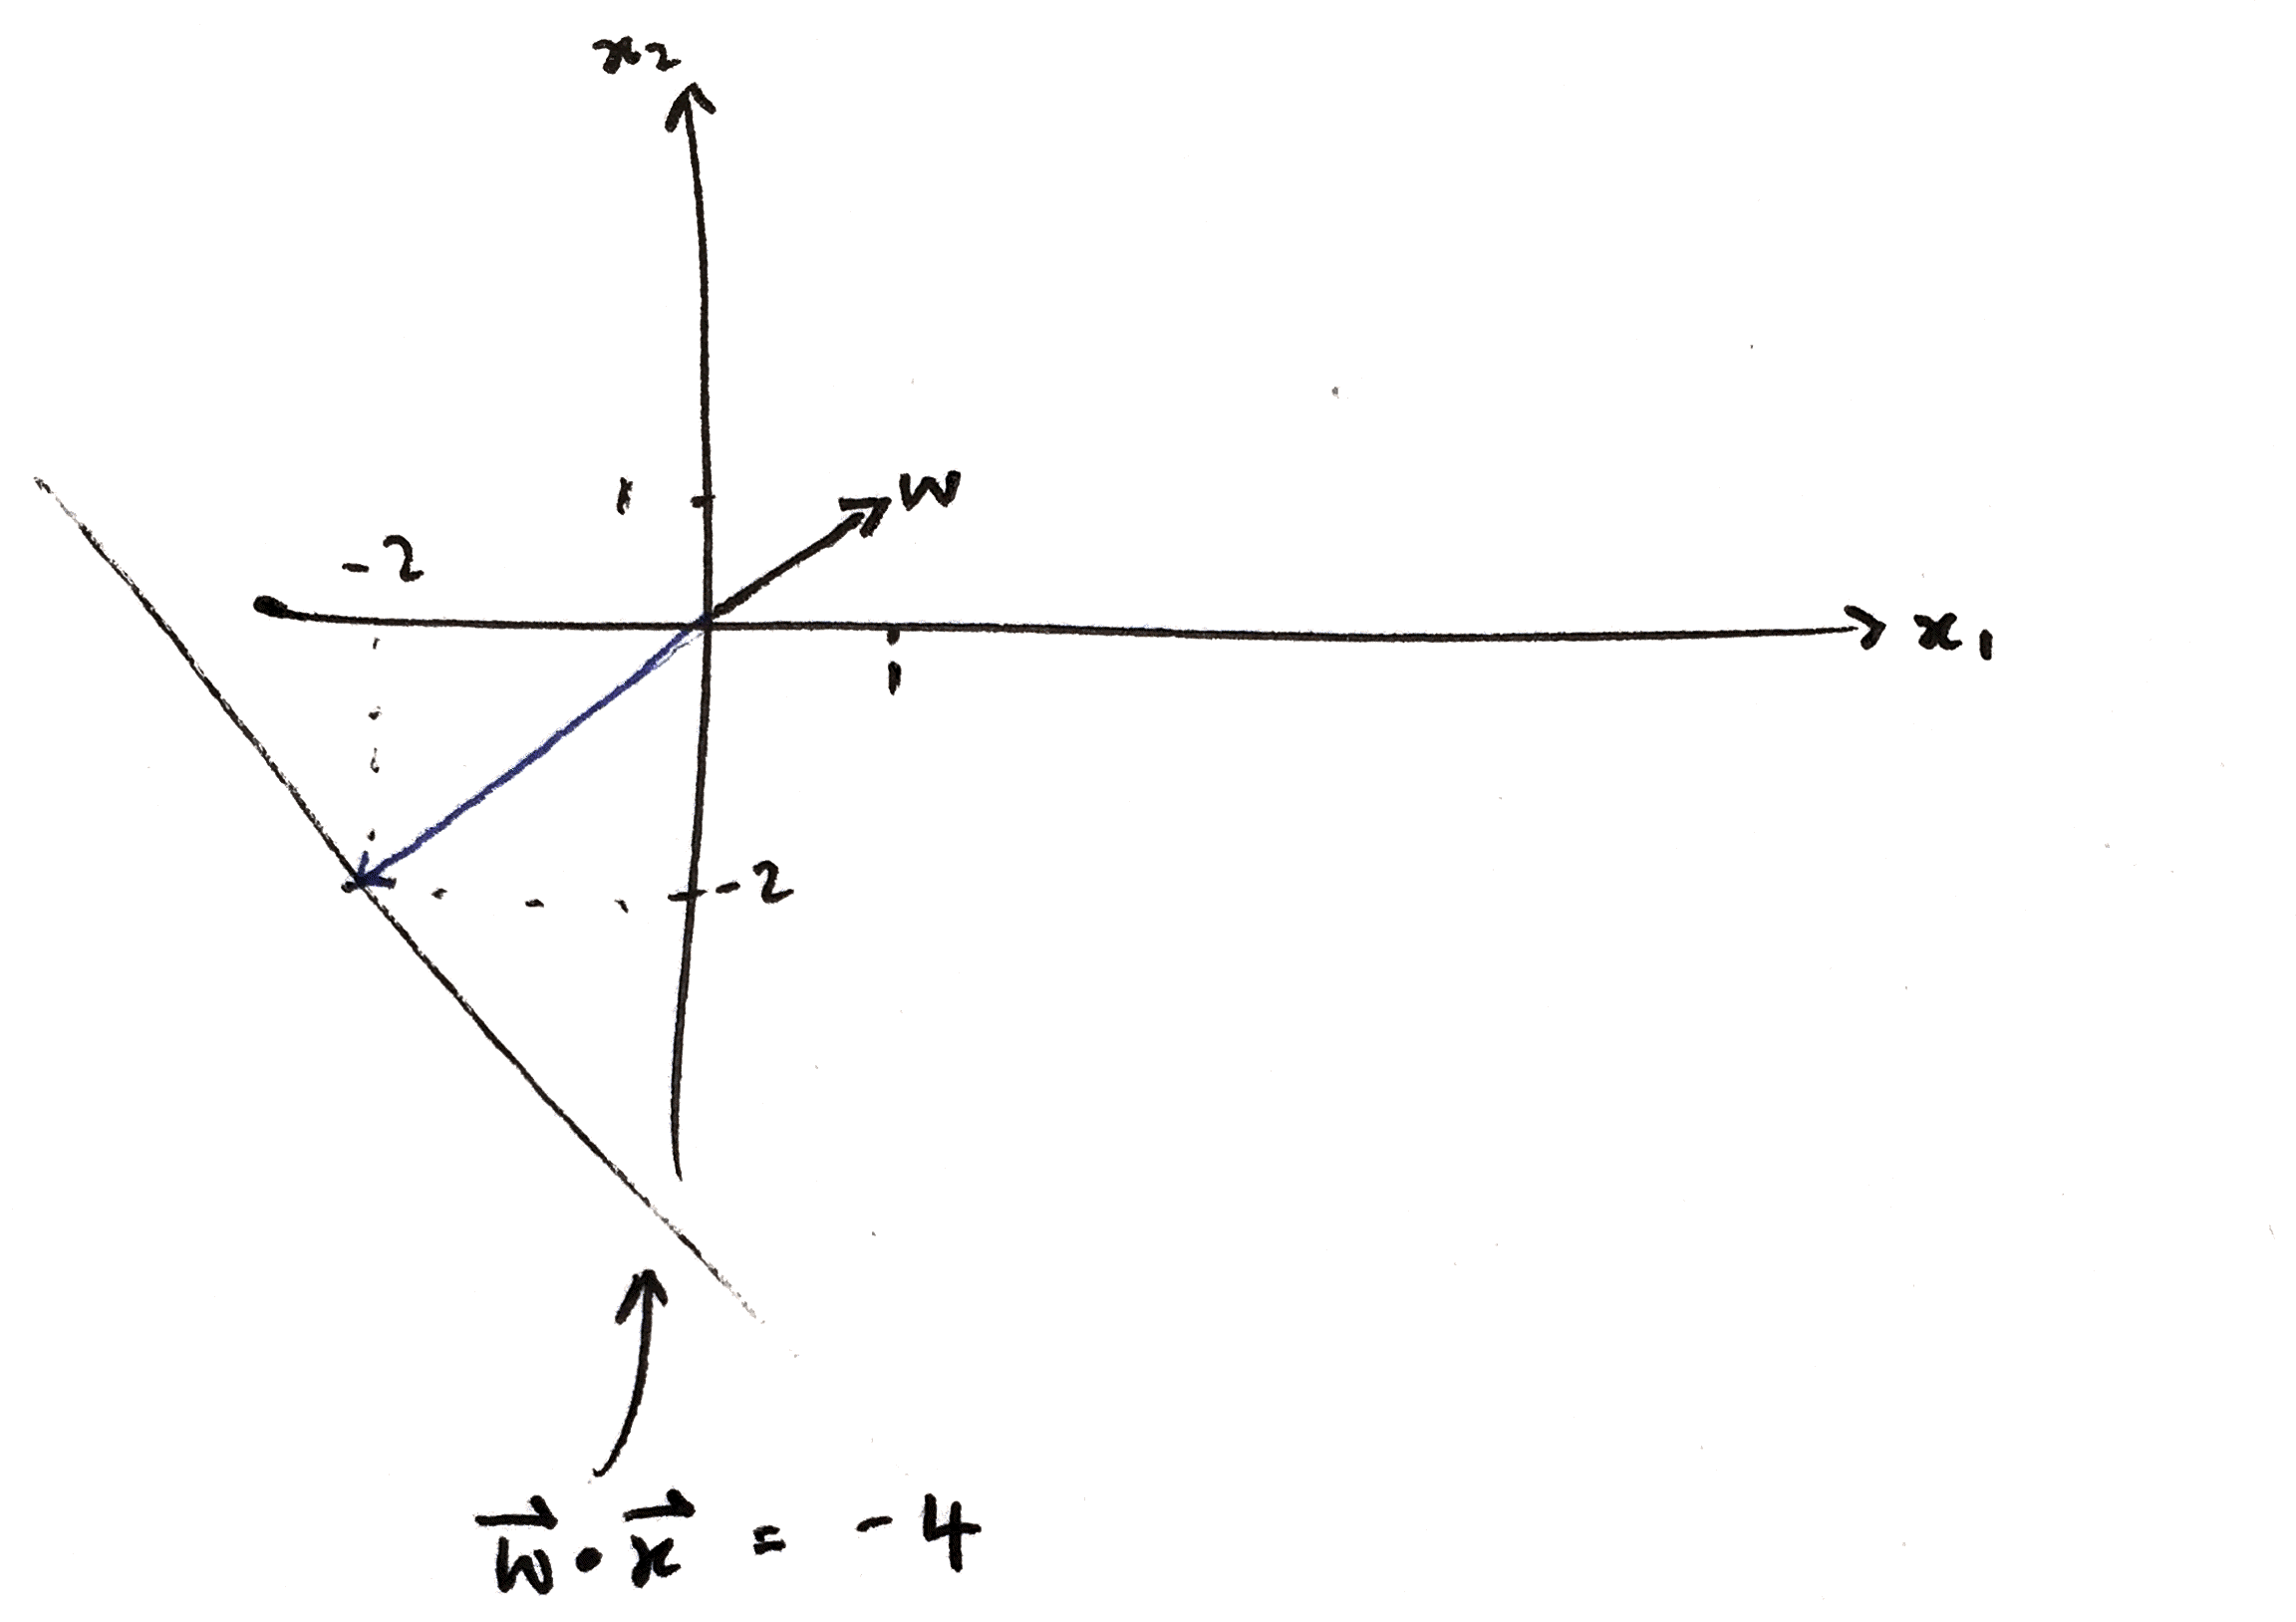
\includegraphics[width=200pt]{img/machine-learning-linear-decision-boundary.png}
\begin{itemize}
\item A plane sloping up at 45° in the north-east direction.
\item Each input feature has equal influence on the classification.
\item Decision boundary is line $x_1 + x_2 = -4$.
\item $\vec w$ is normal to the decision boundary since $\vec w \cdot (\vec x_1 - \vec x_2) = -4 - (-4) = 0$.
\item If one feature has a very high weight then $\vec w$ points close to that
  axis and the decision boundary is almost perpendicular to that axis (other
  features almost don't matter).
\end{itemize}

Examples of linear classifiers:
\begin{description}
\item[Centroid method] Decision boundary perpendicular to and bisects line
  connecting means of labeled training points.
\item[Perceptron]
\item[LDA] Fit Gaussians to each class, same covariance across classes.
\end{description}




\end{document}
